\documentclass{article}

\usepackage[utf8]{inputenc} % For use with utf8 encoding (e.g. é) - note that this is not necessary in Overleaf
\usepackage[letterpaper, margin=1.1in, head=20.1pt]{geometry} % geometry package for greater control over the margins; specify margins of 1 inch and letterpaper (8.5 x 11), along with a longer heading
\usepackage[doublespacing]{setspace} % Set double spacing
\usepackage{graphicx} % Necessary for inserting graphics

% For citations - here using chicago style
\usepackage[authordate-trad,backend=biber]{biblatex-chicago} 
\addbibresource{MyLibrary.bib} % Specify where your .bib file (from Zotero!) is

% Headers and footers
\usepackage{scrlayer-scrpage} % package for improved footers and headers
\clearpairofpagestyles % clear all defaults (location of page #)
\lofoot{Aengus Bridgman} % left footer
\rofoot{Page \thepage} % right footer, page number
\rohead{Introduction to LaTeX} % right, header

\setlength{\textfloatsep}{5pt} % changes the after-figure padding - see the caption or layout packages for more functionality

\newcommand{\mylipsum}{Neque porro quisquam est qui dolorem ipsum quia dolor sit amet, consectetur, adipisci velit...} % Create a command we can draw upon later to produce this text...

% Turn footnotes into endnotes
% \usepackage{endnotes}
% \let\footnote=\endnote

\usepackage{blindtext} % For sample text with \blindtext, \Blindtext, \blinddocument
\usepackage{lipsum} % Another sample text with \lipsum[3-4]

% Three packages for nice tables and figures
\usepackage{booktabs}
\usepackage{dcolumn} 
\usepackage{wrapfig} 
\usepackage{subfig} % For multiple figures side-by-side

%%%%%%%%%%%%%%%%%%%%%%%%%%%%%%%%%%%%%%%%%%%%%%%%%%%%%%%%%%%%%%%%%%%%%%%

\begin{document} % all documents start with a \begin{document}

Welcome to my introduction to LaTeX document. I will teach you to do five common tasks: lists, figures, tables, cross-referencing and footnotes/endnotes, and finally citations. LaTeX has a bit of a learning curve and can be intimidating at first, but once you learn the basics it can help you create beautiful documents and presentations will little effort. It has excellent functionality for math equations and automatic updating while you are tinkering with your plots and tables in the statistical package of your choosing. 

To do something beyond just writing plain text in LaTeX, you write \textbackslash <text> and pass the needed arguments (similar to functions in both Stata and R). For example, if you want to bold text, you just do \textbackslash textbf: \textbf{here is some bolded text}. Command-B works just fine in Overleaf and most LaTeX editors as well. Similarly, for italicized text you do \textbackslash textit \textit{to produce some italicized text.}

\section{Lists} 

Creating lists is a great first exercise for learning LaTeX. We are going to create a small itemize environment and put in the items in our list:

% Create list
\begin{itemize} 
  \item First bullet
  \item Second bullet
  \item Third bullet
\end{itemize}

\noindent We may want instead to have an enumerated list - and let us also make it single spacing:
% Create enumerated list
\begin{enumerate} % For list of items
	\singlespacing % if you assign single spacing within a \begin \end pair, it will only apply within that environment
  \item First item of interest
  \item Second item of interest
  \item Third item of interest
\end{enumerate}

\noindent Or dream big and create a list within a list:
\begin{itemize} % For bullet points
	\singlespacing
  \item First bullet
    \begin{enumerate} % For list of items
    \item Number 1
    \item Number 2
    \item Number 3
 	\end{enumerate}
  \item Second bullet
  \item Third bullet
\end{itemize}

\newpage 
\section*{Figures} % The asterisk removes the section number

One great advantage of LaTeX is that it plays very well with plots and tables exported from Stata and R - without the hassle of resizing every time you change your code slightly. We have a simple plot loaded into the Overleaf environment that we can load using our \textbf{includegraphics} command.

\begin{figure}[!ht]
	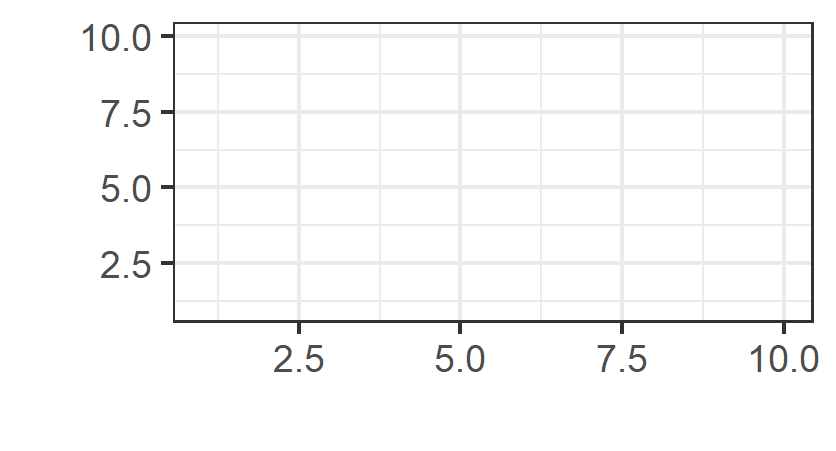
\includegraphics{figures/plot.png}
\end{figure}

That is much too small! If we want to change the size, we add a width or height option to our command. This is the first option we have used - it is kind of like adding additional arguments to a Stata or R function. You do that using arguments in square brackets [], separated by commas.

\begin{figure}[!ht]
	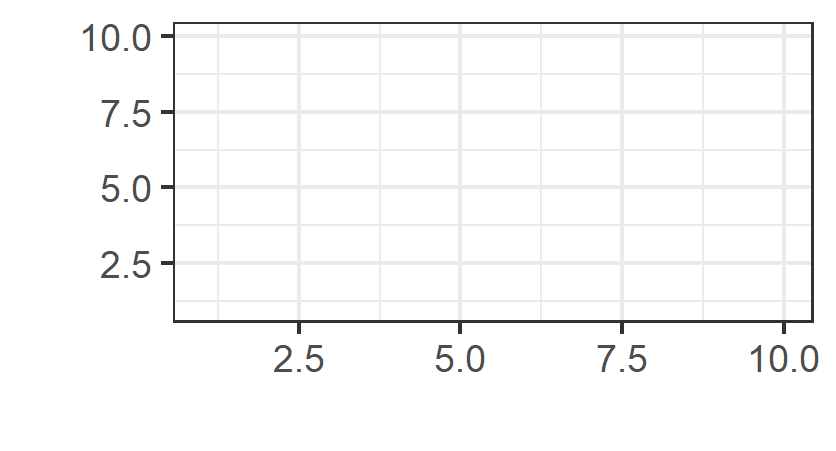
\includegraphics[width=4in]{figures/plot.png}
\end{figure}

\newpage We may want to center the plot:

\begin{figure}[!ht]
	\centering
	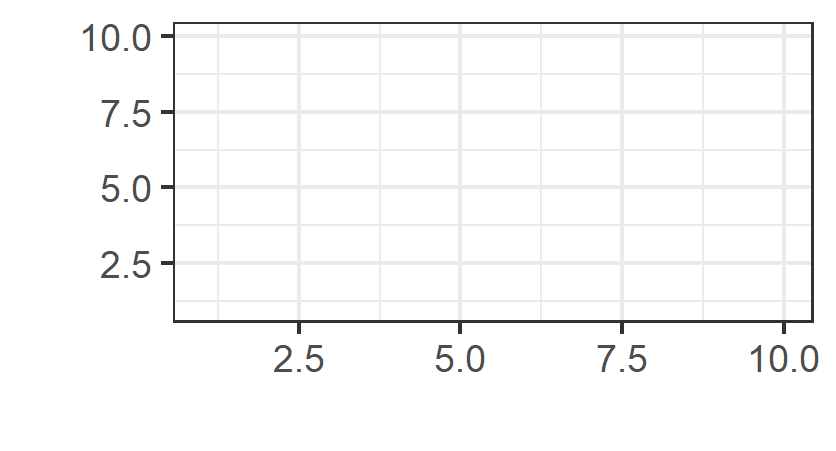
\includegraphics[width=3.6in]{figures/plot.png}
\end{figure}

Add a caption:

\begin{figure}[!ht]
	\centering
    \caption{What a plot!}
	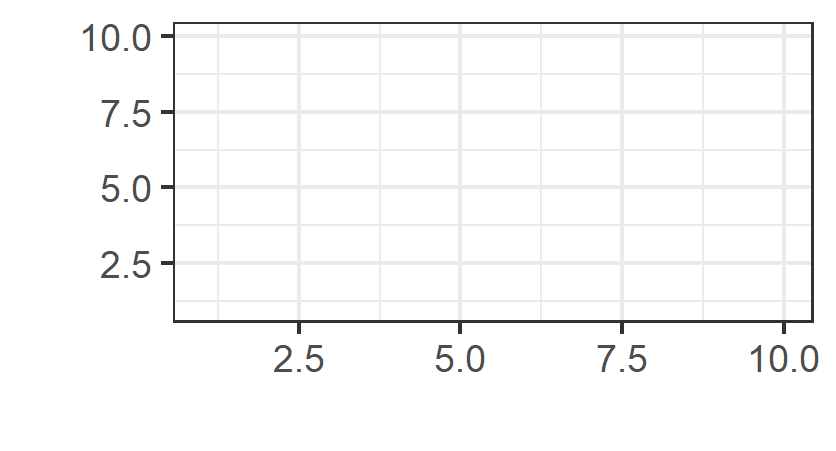
\includegraphics[width=3.6in]{figures/plot.png}
\end{figure}

Or even put two plots side-by-side (although I recommend you do this before-hand):

\begin{figure}[ht]
    \centering
    \subfloat[Plot 1]{{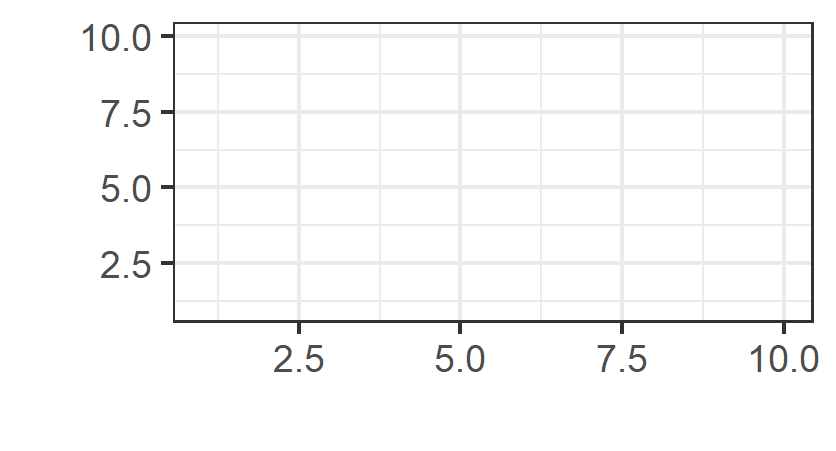
\includegraphics[width=7cm]{figures/plot.png} }}
    \qquad
    \subfloat[Plot 2]{{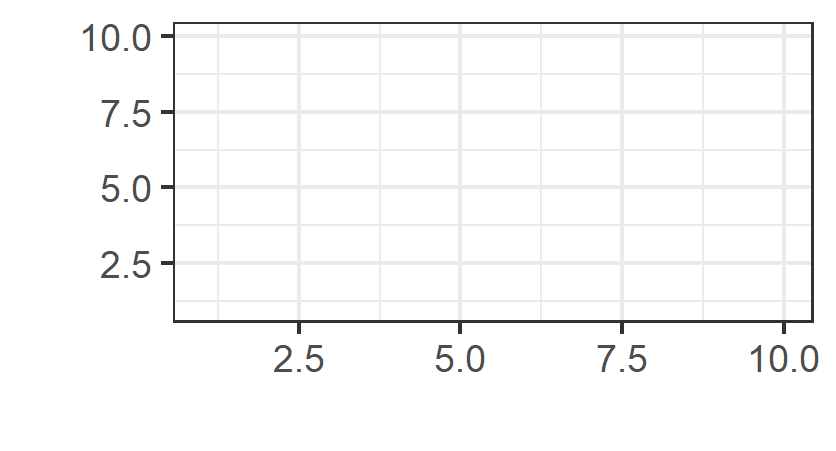
\includegraphics[width=7cm]{figures/plot.png} }}
    \caption{Two plots side by side}
\end{figure}


\newpage 
\section{Tables}

Okay - I am not going to lie - LaTeX tables are an absolute pain if you are producing them by hand. But both Stata and R can produce beautiful tables with functions like texreg, stargazer, latex in R and Esttab in Stata. If you lose your senses and want to create a table this is what something basic looks like:

\begin{center}
  \begin{tabular}{||c c c c||} % c here refers to centered columns
    \hline
    Column & Column & Column & Column \\ % each & breaks up the code between columns
    \hline\hline
    1 & 2 & 3 & 4 \\ 
    \hline
    5 & 6 & 7 & 8 \\
    \hline
  \end{tabular}
\end{center}

\noindent But if you use a statistical software to make a table, it is much easier:

%latex.default(ownership_df, caption = "Perceptions of issue ownership for partisans in Canada for the 2015 federal elections",     label = "partisanownership", booktabs = TRUE, title = "",     cgroup = c("", "Liberal", "Conservative", "NDP"), n.cgroup = c(1,         2, 2, 2), colheads = c("Issue", "Own", "Dif", "Own",         "Dif", "Own", "Dif"), file = paste(save_location, "partisanownership.tex",         sep = ""))%
\begin{table}[!ht]
\caption{Perceptions of issue ownership for partisans in Canada for the 2015 federal elections\label{partisanownership}} 
\begin{center}
\begin{tabular}{llcrrcrrcrr}
\toprule
\multicolumn{1}{l}{\bfseries }&\multicolumn{1}{c}{\bfseries }&\multicolumn{1}{c}{\bfseries }&\multicolumn{2}{c}{\bfseries Liberal}&\multicolumn{1}{c}{\bfseries }&\multicolumn{2}{c}{\bfseries Conservative}&\multicolumn{1}{c}{\bfseries }&\multicolumn{2}{c}{\bfseries NDP}\tabularnewline
\cline{4-5} \cline{7-8} \cline{10-11}
\multicolumn{1}{l}{}&\multicolumn{1}{c}{Issue}&\multicolumn{1}{c}{}&\multicolumn{1}{c}{Own}&\multicolumn{1}{c}{Dif}&\multicolumn{1}{c}{}&\multicolumn{1}{c}{Own}&\multicolumn{1}{c}{Dif}&\multicolumn{1}{c}{}&\multicolumn{1}{c}{Own}&\multicolumn{1}{c}{Dif}\tabularnewline
\midrule
1&Crime&&$54.5$&$22.2$&&$66.2$&$10.5$&&$36.3$&$39.2$\tabularnewline
2&Environment&&$44.0$&$36.9$&&$32.6$&$42.2$&&$32.8$&$50.5$\tabularnewline
3&Defence&&$52.9$&$24.0$&&$68.8$&$ 8.1$&&$29.0$&$45.3$\tabularnewline
4&Immigration&&$64.6$&$12.1$&&$49.6$&$23.5$&&$44.0$&$30.9$\tabularnewline
\bottomrule
\end{tabular}\end{center}
\end{table}


\noindent And you have to do much less work on the LaTeX end

%latex.default(stat_table_2, caption = "Vote ownership, salience and diffentiation summary table for major political parties in the 2015 federal election",     rowlabel = "", booktabs = TRUE, title = "", n.rgroup = c(5,         5, 5), n.cgroup = c(3, 3), center = "centerline", cgroup = c("",         "Salience"), rgroup = c("Lib", "Con", "NDP"), file = paste(save_location,         "stat_table.tex", sep = ""))%
\begin{table}[ht]
\caption{Voter ownership, salience and party differentiation summary table for major political parties in the 2015 federal election\label{}} 
\centerline{\begin{tabular}{llrrcrrr}
\toprule
\multicolumn{1}{l}{\bfseries }&\multicolumn{3}{c}{\bfseries }&\multicolumn{1}{c}{\bfseries }&\multicolumn{3}{c}{\bfseries Salience (\%)}\tabularnewline
\cline{6-8}
\multicolumn{1}{l}{}&\multicolumn{1}{c}{Issue}&\multicolumn{1}{c}{Party (\%)}&\multicolumn{1}{c}{Voters (\%)}&\multicolumn{1}{c}{}&\multicolumn{1}{c}{High}&\multicolumn{1}{c}{Low}&\multicolumn{1}{c}{No}\tabularnewline
\midrule
{\bfseries Lib}&&&&&&&\tabularnewline
~~&Environment&$48.25$&$51.59$&&$45.17$&$47.23$&$ 7.60$\tabularnewline
~~&Crime&$19.62$&$41.60$&&$40.13$&$50.71$&$ 9.16$\tabularnewline
~~&Defence&$30.54$&$39.83$&&$26.86$&$53.54$&$19.60$\tabularnewline
~~&Immigration&$17.42$&$53.89$&&$50.19$&$40.13$&$ 9.68$\tabularnewline
\midrule
{\bfseries Con}&&&&&&&\tabularnewline
~~&Environment&$20.38$&$22.40$&&$29.71$&$55.23$&$15.06$\tabularnewline
~~&Crime&$68.89$&$44.19$&&$50.21$&$43.50$&$ 6.29$\tabularnewline
~~&Defence&$60.45$&$48.70$&&$37.47$&$48.23$&$14.30$\tabularnewline
~~&Immigration&$62.13$&$21.58$&&$38.29$&$48.10$&$13.61$\tabularnewline
\midrule
{\bfseries NDP}&&&&&&&\tabularnewline
~~&Environment&$31.37$&$26.01$&&$51.92$&$42.86$&$ 5.23$\tabularnewline
~~&Crime&$11.49$&$14.21$&&$37.14$&$53.06$&$ 9.80$\tabularnewline
~~&Defence&$ 9.01$&$11.47$&&$23.56$&$54.68$&$21.76$\tabularnewline
~~&Immigration&$20.44$&$24.53$&&$48.66$&$41.09$&$10.24$\tabularnewline
\bottomrule
\end{tabular}}
\end{table}


\newpage \section{Cross-referencing and footnotes/endnotes} % Can put multiple commands on a single line

If I want to reference another place in the document I can use the ref command. For example, I want to reference Section~\ref{sec:citations} on page~\pageref{sec:citations}. I may also want to reference a particular figure. But I can only do that if there is a \textbackslash label that identifies a figure. Go ahead and reference a table or figure we identified earlier (hint: put the \textbackslash label into the environment created for the table or figure). 

Footnotes are easy to do in LaTeX: just use \textbackslash footnote. \footnote{I can also be made into an endnote easily!}

\newpage 
\section{References} \label{sec:citations} % Have created a label for this section

\begin{itemize}
  \item First I do a straight citation: \cite{blais_vote_2000} % straight citation
  \item But convention is normally to have parentheses around a citation: \parencite{kymlicka_multicultural_1995} % citation in parentheses
  \item Sometimes I want to directly refer to a page number: \parencite[p. 10]{gidengil_dominance_2012} % citation with [page after]
  \item Or have both before and after text: \parencite[see for example][pp. 8-15]{stolle_getting_2001} % \parencite[first text][second text]{code}
    \item If perhaps I don't want the author's name to appear, then I add as asterisk: \parencite*{fournier_when_2011} 
\end{itemize}

That is all for the basics for an article! See the included file for a full example paper written in LaTeX with dummy text.

% Put in endnotes
% \clearpage \singlespacing
% \theendnotes

% Insert bibliography
\clearpage \singlespacing % stronger page break - removes formatting as well
\printbibliography % prints the bibliography

\end{document}
